\chapter{Air Separation Technology}
\label{chp:airsep}
\begin{figure}[h]
	\begingroup%
  \makeatletter%
    \setlength{\unitlength}{1cm}%
  \makeatother%
  \begin{picture}(17, 7)%	
    \scriptsize
    \put(2,1){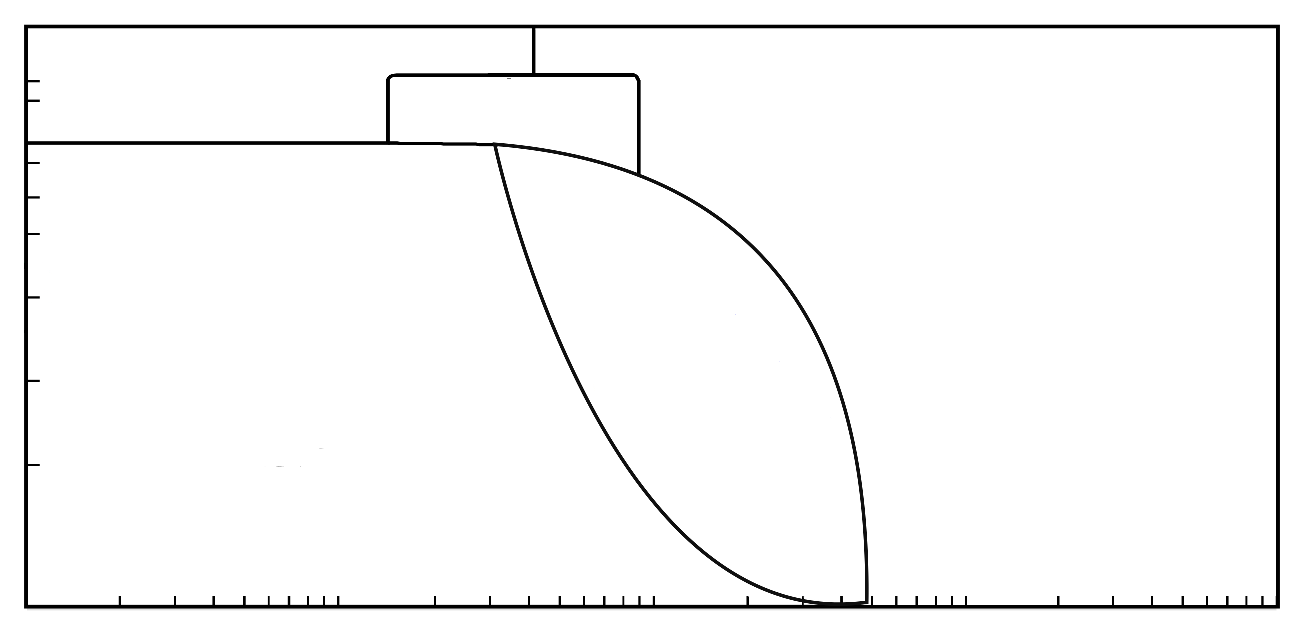
\includegraphics[width=13cm]{Pictures/tech_comp_graph.eps}}%
    \put(8.5, 0.1){\color[rgb]{0,0,0}\makebox(0,0)[c]{\smash{\normalsize{product stream $[\frac{m^3_{STP}}{h}]$}}}}%
    \put(0.6, 4){\color[rgb]{0,0,0}\rotatebox{90}{\makebox(0,0)[c]{\smash{\normalsize{$N_2$-purity $x_{N_2, Ret}$ $[\%]$}}}}}%
    \put(1.9, 0.65){\color[rgb]{0,0,0}\makebox(0,0)[l]{\smash{$10$}}}%
    \put(5.15, 0.65){\color[rgb]{0,0,0}\makebox(0,0)[l]{\smash{$10^2$}}}%
    \put(8.35, 0.65){\color[rgb]{0,0,0}\makebox(0,0)[l]{\smash{$10^3$}}}%
    \put(11.55, 0.65){\color[rgb]{0,0,0}\makebox(0,0)[l]{\smash{$10^4$}}}%
    \put(14.75, 0.65){\color[rgb]{0,0,0}\makebox(0,0)[l]{\smash{$10^5$}}}%
    \put(1.85, 1){\color[rgb]{0,0,0}\makebox(0,0)[r]{\smash{$95$}}}%
    \put(1.85, 2.45){\color[rgb]{0,0,0}\makebox(0,0)[r]{\smash{$97$}}}%
    \put(1.85, 3.325){\color[rgb]{0,0,0}\makebox(0,0)[r]{\smash{$98$}}}%
    \put(1.85, 4.15){\color[rgb]{0,0,0}\makebox(0,0)[r]{\smash{$99$}}}%
    \put(1.85, 4.8){\color[rgb]{0,0,0}\makebox(0,0)[r]{\smash{$99.5$}}}%
    \put(1.85, 5.2){\color[rgb]{0,0,0}\makebox(0,0)[r]{\smash{$99.9$}}}%
    \put(1.85, 5.55){\color[rgb]{0,0,0}\makebox(0,0)[r]{\smash{$99.95$}}}%
    \put(1.85, 6.1){\color[rgb]{0,0,0}\makebox(0,0)[r]{\smash{$99.99$}}}%
    \put(1.85, 6.4){\color[rgb]{0,0,0}\makebox(0,0)[r]{\smash{$99.999$}}}%
    \put(1.85, 6.4){\color[rgb]{0,0,0}\makebox(0,0)[r]{\smash{}}}%
    \put(5,3){\color[rgb]{0,0,0}\normalsize{\CM{membrane processes / \\ gas permeation}}}%
    \put(8.9,3.7){\color[rgb]{0,0,0}\normalsize{\CM{PSA}}}%
    \put(7,6.20){\color[rgb]{0,0,0}\scriptsize{\CM{membrane \& \\ post oxidation}}}%
    \put(4,6.5){\color[rgb]{0,0,0}\normalsize{\CM{cryogenic processes \\ (liquid)}}}%
    \put(12,5.5){\color[rgb]{0,0,0}\normalsize{\CM{cryogenic processes \\ (gaseous)}}}%
  \end{picture}%
\endgroup%

	\caption{Comparison of Air Separation Technologies \cite{Prasad.1994}.}
	\label{fig:tech_compar}
\end{figure}

There are several ways besides cryogenic air separation that can be employed to separate gas mixtures. 
In this chapter different competing technologies and their main applications will be discussed. The 
predominately used technologies are cryogenic distillation, pressure swing adsorption (PSA) as well as 
gas permeation (GP). In the distillation process the gas is first liquefied. Separation is the achieved 
by the different concentration differences in vapor and liquid phase. PSA relies on the different affinities 
of gaseous species to adsorb to certain materials in order to extract a component form a mixture. During gas 
permeation membranes are used. Each species migrates in different quantities through a given membrane
depending on process parameters and membrane structure. 

\reffig{fig:tech_compar} illustrates the most economically viable processes depending on product
purity and product stream volume. It can be seen that alternative air separation processes 
cannot supply the high quality or quantity of the cryogenic process. Due to that cryogenic air separation is 
thought to be the main supplier of highly pure gases in industrial quantities for years to come 
\cite{Castle.2002}. 
The alternative processes however offer some very appealing characteristics, which make them the 
favorable choice when lower quantities of product or more moderate purity is required. The cryogenic 
process is always connected with an considerable energy consumption for the liquefaction and compression. 
Due to that smaller implementations of the process a very unlikely to yield economically sound solutions
to a separation problem. 

\addref

\section{Cryogenic Air Separation}
\label{sec:cryo_air_sep}
Cryogenic Air Separation finds applications over a great variety of industries among others refining, petrochemicals, medical, food \& beverages and environmental \cite{Sirdeshpande.2005}. Furthermore 
prospective processes for power generation from fossil sources in form of the integrated gaseous combined 
cycle (IGCC) integrates the air separation process in order to enable more environmentally friendly power 
generation \cite{Mahapatra.2010}. 

\begin{figure}
	%% Creator: Inkscape inkscape 0.48.2, www.inkscape.org
%% PDF/EPS/PS + LaTeX output extension by Johan Engelen, 2010
%% Accompanies image file 'ASU_text.eps' (pdf, eps, ps)
%%
%% To include the image in your LaTeX document, write
%%   \input{<filename>.pdf_tex}
%%  instead of
%%   \includegraphics{<filename>.pdf}
%% To scale the image, write
%%   \def\svgwidth{<desired width>}
%%   \input{<filename>.pdf_tex}
%%  instead of
%%   \includegraphics[width=<desired width>]{<filename>.pdf}
%%
%% Images with a different path to the parent latex file can
%% be accessed with the `import' package (which may need to be
%% installed) using
%%   \usepackage{import}
%% in the preamble, and then including the image with
%%   \import{<path to file>}{<filename>.pdf_tex}
%% Alternatively, one can specify
%%   \graphicspath{{<path to file>/}}
%% 
%% For more information, please see info/svg-inkscape on CTAN:
%%   http://tug.ctan.org/tex-archive/info/svg-inkscape
%%
\begingroup%
  \makeatletter%
  \providecommand\color[2][]{%
    \errmessage{(Inkscape) Color is used for the text in Inkscape, but the package 'color.sty' is not loaded}%
    \renewcommand\color[2][]{}%
  }%
  \providecommand\transparent[1]{%
    \errmessage{(Inkscape) Transparency is used (non-zero) for the text in Inkscape, but the package 'transparent.sty' is not loaded}%
    \renewcommand\transparent[1]{}%
  }%
  \providecommand\rotatebox[2]{#2}%
  \ifx\svgwidth\undefined%
    \setlength{\unitlength}{480.89958443bp}%
    \ifx\svgscale\undefined%
      \relax%
    \else%
      \setlength{\unitlength}{\unitlength * \real{\svgscale}}%
    \fi%
  \else%
    \setlength{\unitlength}{\svgwidth}%
  \fi%
  \global\let\svgwidth\undefined%
  \global\let\svgscale\undefined%
  \makeatother%
  \begin{picture}(1,0.69511554)%
    \scriptsize		
    \put(0,0){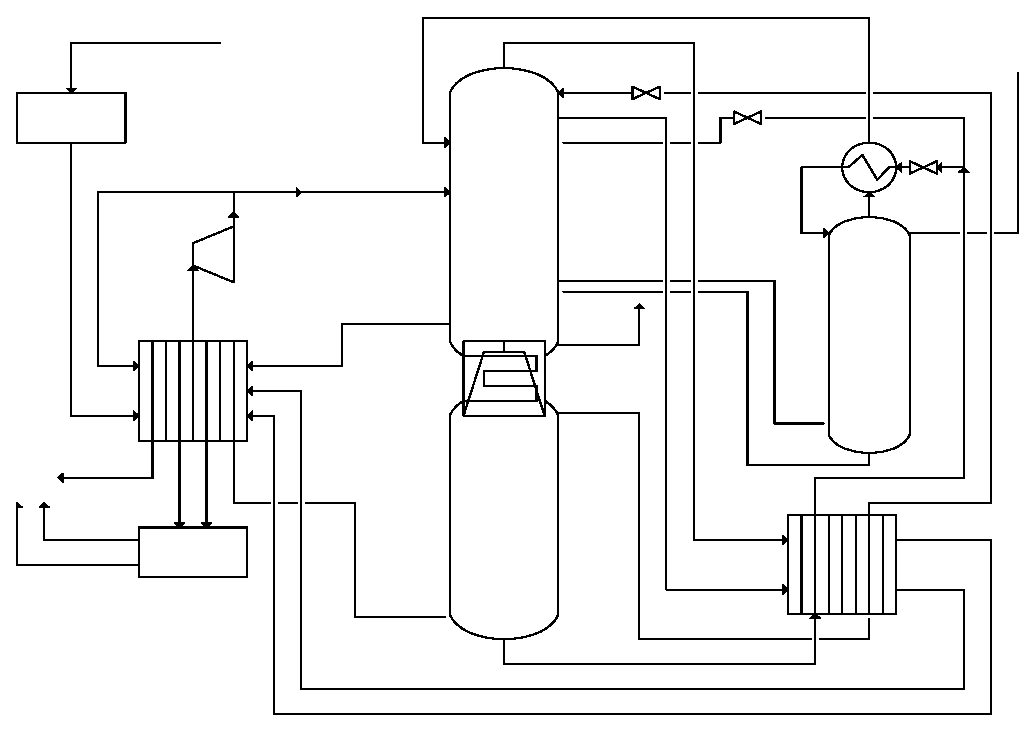
\includegraphics[width=\unitlength]{Pictures/ASU_text.eps}}%
    \put(0.47303574,0.48730942){\color[rgb]{0,0,0}\makebox(0,0)[lb]{\smash{LPC}}}%
    \put(0.4694296,0.20132682){\color[rgb]{0,0,0}\makebox(0,0)[lb]{\smash{HPC}}}%
    \put(0.83500402,0.38163476){\color[rgb]{0,0,0}\makebox(0,0)[lb]{\smash{CAC}}}%
    \put(0.05258426,0.59980743){\color[rgb]{0,0,0}\CM{compression \& \\ pre-purification}}%
    \put(0.14352294,0.15715136){\color[rgb]{0,0,0}\makebox(0,0)[lb]{\smash{liquefier}}}%
    \put(0.29858781,0.52588116){\color[rgb]{0,0,0}\makebox(0,0)[lb]{\smash{expanded air}}}%
    \put(0.38899094,0.33926244){\color[rgb]{0,0,0}\CM{condenser / \\�re-boiler}}%
    \put(0.32743709,0.39696094){\color[rgb]{0,0,0}\makebox(0,0)[lb]{\smash{gas oxygen}}}%
    \put(0.54290509,0.35549012){\color[rgb]{0,0,0}\makebox(0,0)[lb]{\smash{liquid oxygen}}}%
    \put(0.5699513,0.05437579){\color[rgb]{0,0,0}\makebox(0,0)[lb]{\smash{oxygen-rich liquid}}}%
    \put(0.59339131,0.00479107){\color[rgb]{0,0,0}\makebox(0,0)[lb]{\smash{gas nitrogen}}}%
    \put(0.99337587,0.51282048){\color[rgb]{0,0,0}\rotatebox{90}{\makebox(0,0)[lb]{\smash{crude argon}}}}%
    \put(0.58437597,0.03003421){\color[rgb]{0,0,0}\makebox(0,0)[lb]{\smash{waste nitrogen}}}%
    \put(0.54921586,0.43572716){\color[rgb]{0,0,0}\makebox(0,0)[lb]{\smash{argon feed}}}%
    \put(0.74214534,0.25361611){\color[rgb]{0,0,0}\makebox(0,0)[lb]{\smash{argon return}}}%
    \put(0.10115056,0.6764383){\color[rgb]{0,0,0}\makebox(0,0)[lb]{\smash{plant air}}}%
    \put(0.3598925,0.10215738){\color[rgb]{0,0,0}\makebox(0,0)[lb]{\smash{air feed}}}%
    \put(0.53298812,0.67373368){\color[rgb]{0,0,0}\makebox(0,0)[lb]{\smash{gas nitrogen}}}%
    \put(0.54560966,0.60070896){\color[rgb]{0,0,0}\makebox(0,0)[lb]{\smash{waste nitrogen}}}%
    \put(0.12754442,0.3960594){\color[rgb]{0,0,0}\CM{heat \\ exchanger}}%
    \put(0.75059149,0.21935756){\color[rgb]{0,0,0}\CM{heat \\�exchanger}}%
    \put(0.14262141,0.48170568){\color[rgb]{0,0,0}\makebox(0,0)[lb]{\smash{turbine}}}%
    \put(0.66010521,0.0805205){\color[rgb]{0,0,0}\makebox(0,0)[lb]{\smash{liquid nitrogen}}}%
  \end{picture}%
\endgroup%

	\caption[Air Separation Unit]{Schematic representation of the cryogenic air separation process.}
	\label{fig:ASU}
\end{figure}

As can be seen in \reffig{fig:ASU} double effect heat integrated distillation column lies at the heart of the air 
liquefaction processes. It consists of a high pressure column (HPC) operating at 0.68 $MPa$ and 
temperatures below 130 $K$ as well as a low pressure column (LPC) which operates at around 0.13 
$MPa$ an comparable temperatures. In order to also attain highly pure argon as a product the process 
may also include a crude argon column (CAC) which works at slightly lower pressures than the LPC.

The plant air entering the process is initially purified, where carbon and nitrogen oxides as well as solid contaminants are removed, and then compressed to process conditions. The compressed air is then cooled 
against product streams namely liquefied nitrogen, oxygen and argon. The air stream is then divided into 
several sub-streams. One of those is fed into the HPC bottom, while another is expanded by means of a 
turbine and further cooled down through the Joule- Thompson effect. Aside from further cooling energy from 
the initial compression is thus partially recovered. This expanded air stream is then fed into the LPC. At the 
bottom of the LPC liquid as well as gaseous oxygen are recovered as desired products. The bottom and top 
streams from the HPC are made up of an oxygen rich liquid as well as liquid nitrogen. The liquid nitrogen 
stream is led though an heat exchanger an the fed as reflux into the top of the LPC. The bottom stream is, 
after heat integration, partially fed into the LPC as well as CAC. From the lower part of the LPC a side stream 
is drawn and led into the bottom of the CAC. At the same point the reflux from the CAC is fed back into the 
LPC \cite{Zhu.2010}.

\section{Pressure Swing Adsorbtion}
\label{sec:psa}



Pressure Swing Adsorption has been employed to separate gaseous mixtures for some time. During the 
80's and 90's commercial applications for the production of oxygen or nitrogen have gained more and 
more attention. Especially the ability to construct very compact units the size of a briefcase, have led to 
the implementation  of PSA processes for treatment of asthma patients or other medical appliances. But 
also larger scale plants have successfully been utilized, for example in the paper industry during the 
de-lignation of pulp. It remains true however, that for large scale industrial settings with high product 
quality demands, cryogenic separation remains the most viable alternative. 

Separation is achieved during the PSA process by adsorption of one component in the mixture to a given
bed. Once the bed is saturated with a the adsorbing species, it has to be regenerated in order to continue 
production. The ability to adsorb a certain species is dependent on the system pressure. At higher pressures
more gas can be adsorbed then at lower pressures. Thus by reducing the pressure in the reaction vessel, 
the Adsorbent can be regenerated. 

\begin{figure}
	\center
	\begin{tikzpicture}
	\draw [line width = 1pt] (-3,-1.65) -- (0,-1.65) .. controls (0.5,-1.55) and (0.5,-0.55) .. (0,-0.45) --%
		(-3,-0.45) .. controls (-3.5,-0.55) and (-3.5,-1.55) .. (-3,-1.65) -- cycle;
	\draw [line width = 1pt] (-3,0.45) -- (0,0.45) .. controls (0.5,0.55) and (0.5,1.55) .. (0,1.65) --%
		(-3,1.65) .. controls (-3.5,1.55) and (-3.5,0.55) .. (-3,0.45) -- cycle;
	\draw [arrow] (-7,0) -- (-6.5,0) -- (-6.5,-1.05) -- (-6,-1.05);
	\pgfvalveh{-6}{-1.05}
	\draw [arrow] (-6.5,0) -- (-6.5,1.05) -- (-6,1.05);
	\pgfvalveh{-6}{1.05}
\end{tikzpicture}

	\caption{Schematic representation of the PSA process.}
	\label{fig:PSA}
\end{figure}

In order to avoid non-continuous processes, two or more reaction vessels are employed. Therefore the 
saturated vessel can be regenerated, while the other one continues production. By alternating adsorption 
and regenerating in the different vessels continuous production can be achieved. A schematic for a simple 
two bed cycle is shown in \reffig{fig:PSA}. Ambient air is first led through the first reaction vessel at the 
elevated pressure. Within the vessel nitrogen is adsorbed until saturation is reached. At that point the 
ambient air is led through the second vessel. A fraction of the product stream is fed into the first vessel and 
used as sweep for the regeneration of the adsorbent at lower pressure. 

Depending on the size of the process two different pressure level are used. One cycle adsorbs the nitrogen 
at a pressure of approximately  7.5 bar while regeneration is done at ambient pressure. Within the 
alternative approach adsorption occurs under ambient condition, while for the regeneration step a vacuum 
pump reduces the vessel pressure. This process is the called Vacuum Pressure Swing Adsorption (VPSA). 

An important role when designing the product is the choice of the adsorbent. For almost all current 
applications of PSA alumosilicates or zeolithes have been designed, tailored to the specific separation 
task. Their main advantages include a high selectivity towards a specic gas to be adsorbed as well as a 
very homogenous distribution of diameters in the molecular sieve. 

\section{Gas Permeation}
\label{sec:membrane}
\todo[inline]{find paper: DOI: 10.1002/cite.330480804}
\todo[inline]{add reference: ISBN-10: 354034327X}
The separation of mixed gases by membrane process is called gas permeation. Its main strength 
in comparison with alternative processes are the low energy consumption and the possibility to 
produce flexible mobile units. As mentioned before it is not however capable of producing high
quantity highly pure product streams. As \reffig{fig:tech_compar} illustrates the main application 
for the gas permeation process are small to moderate product streams at intermediate purities.   

\begin{figure}
	\center
	
\begingroup%
  \makeatletter%
    \setlength{\unitlength}{1cm}%
  \makeatother%
  \begin{picture}(13, 7)%	
    \put(0,0){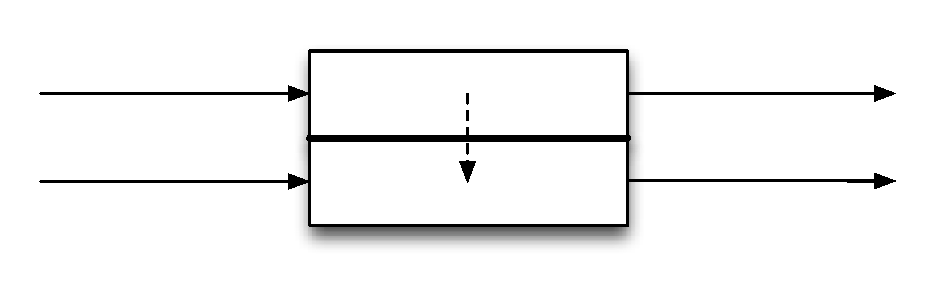
\includegraphics[width=13cm]{Pictures/gas_permeation.eps}}%
    \put(2.3, 1.5){\color[rgb]{0,0,0}\makebox(0,0)[c]{\smash{sweep}}}%
     \put(2.3, 2.8){\color[rgb]{0,0,0}\makebox(0,0)[c]{\smash{feed}}}%
     \put(10.7, 1.5){\color[rgb]{0,0,0}\makebox(0,0)[c]{\smash{retentate}}}%
     \put(10.7, 2.8){\color[rgb]{0,0,0}\makebox(0,0)[c]{\smash{permeate}}}%
  \end{picture}%
\endgroup%

	\caption{Gas permeation process.}
	\label{fig:gas_permeation} 
\end{figure}

\reffig{fig:gas_permeation} shows the schematic for a single stage membrane unit. Within the feed stream 
the gaseous mixture is fed into the unit, which can quickly be implemented. Within the unit one or more 
species migrate favorably through the membrane. In this case mostly dense polymer membranes are 
employed used. There have been some impressive results with metallic membranes, but due to 
the very high material costs they have not been adapted by the industry. Furthermore, since gaseous 
phases often have rather small molecular species, porous membranes cannot achieve desired separation. 
The driving force the separation process is a difference in partial pressure or species activity across the 
membrane. According to the molecular structure of each species, the structure of the separating membrane 
as well as the process parameters pressure and temperature, they permeate through the membrane in 
different quantities.

The process of permeation can be subdivided into three separate steps. Sorption at the membrane / 
feed interface, diffusion through the mostly dense polymer membrane and finally desorption at the 
permeate side of the membrane. 
